\section{Report Task}
\textbf{Combine, within a single image, a rendered portion of the volumetric dataset together with the anatomical 2D views, the various measurements or markups generated in the previous task and the models generated from the segmentation task. Create meaningful visualizations that would enable a hypothetical medical expert to gain insights into the key regions of interest within the examined volumetric model. Imagine that these visualizations (snapshots) will be included as part of a report prepared for such an expert.}\\

Using the segmentation model generated in task 1, we generated meaningful visualizations of the model and the markups. This capture enables the doctor to clearly analyze the structure and shape of the lungs, as well as seeing the various lung measurements

As we already had the segmentation and the markups done, the process was very straightforward.

\begin{figure}[H]
    \centering
    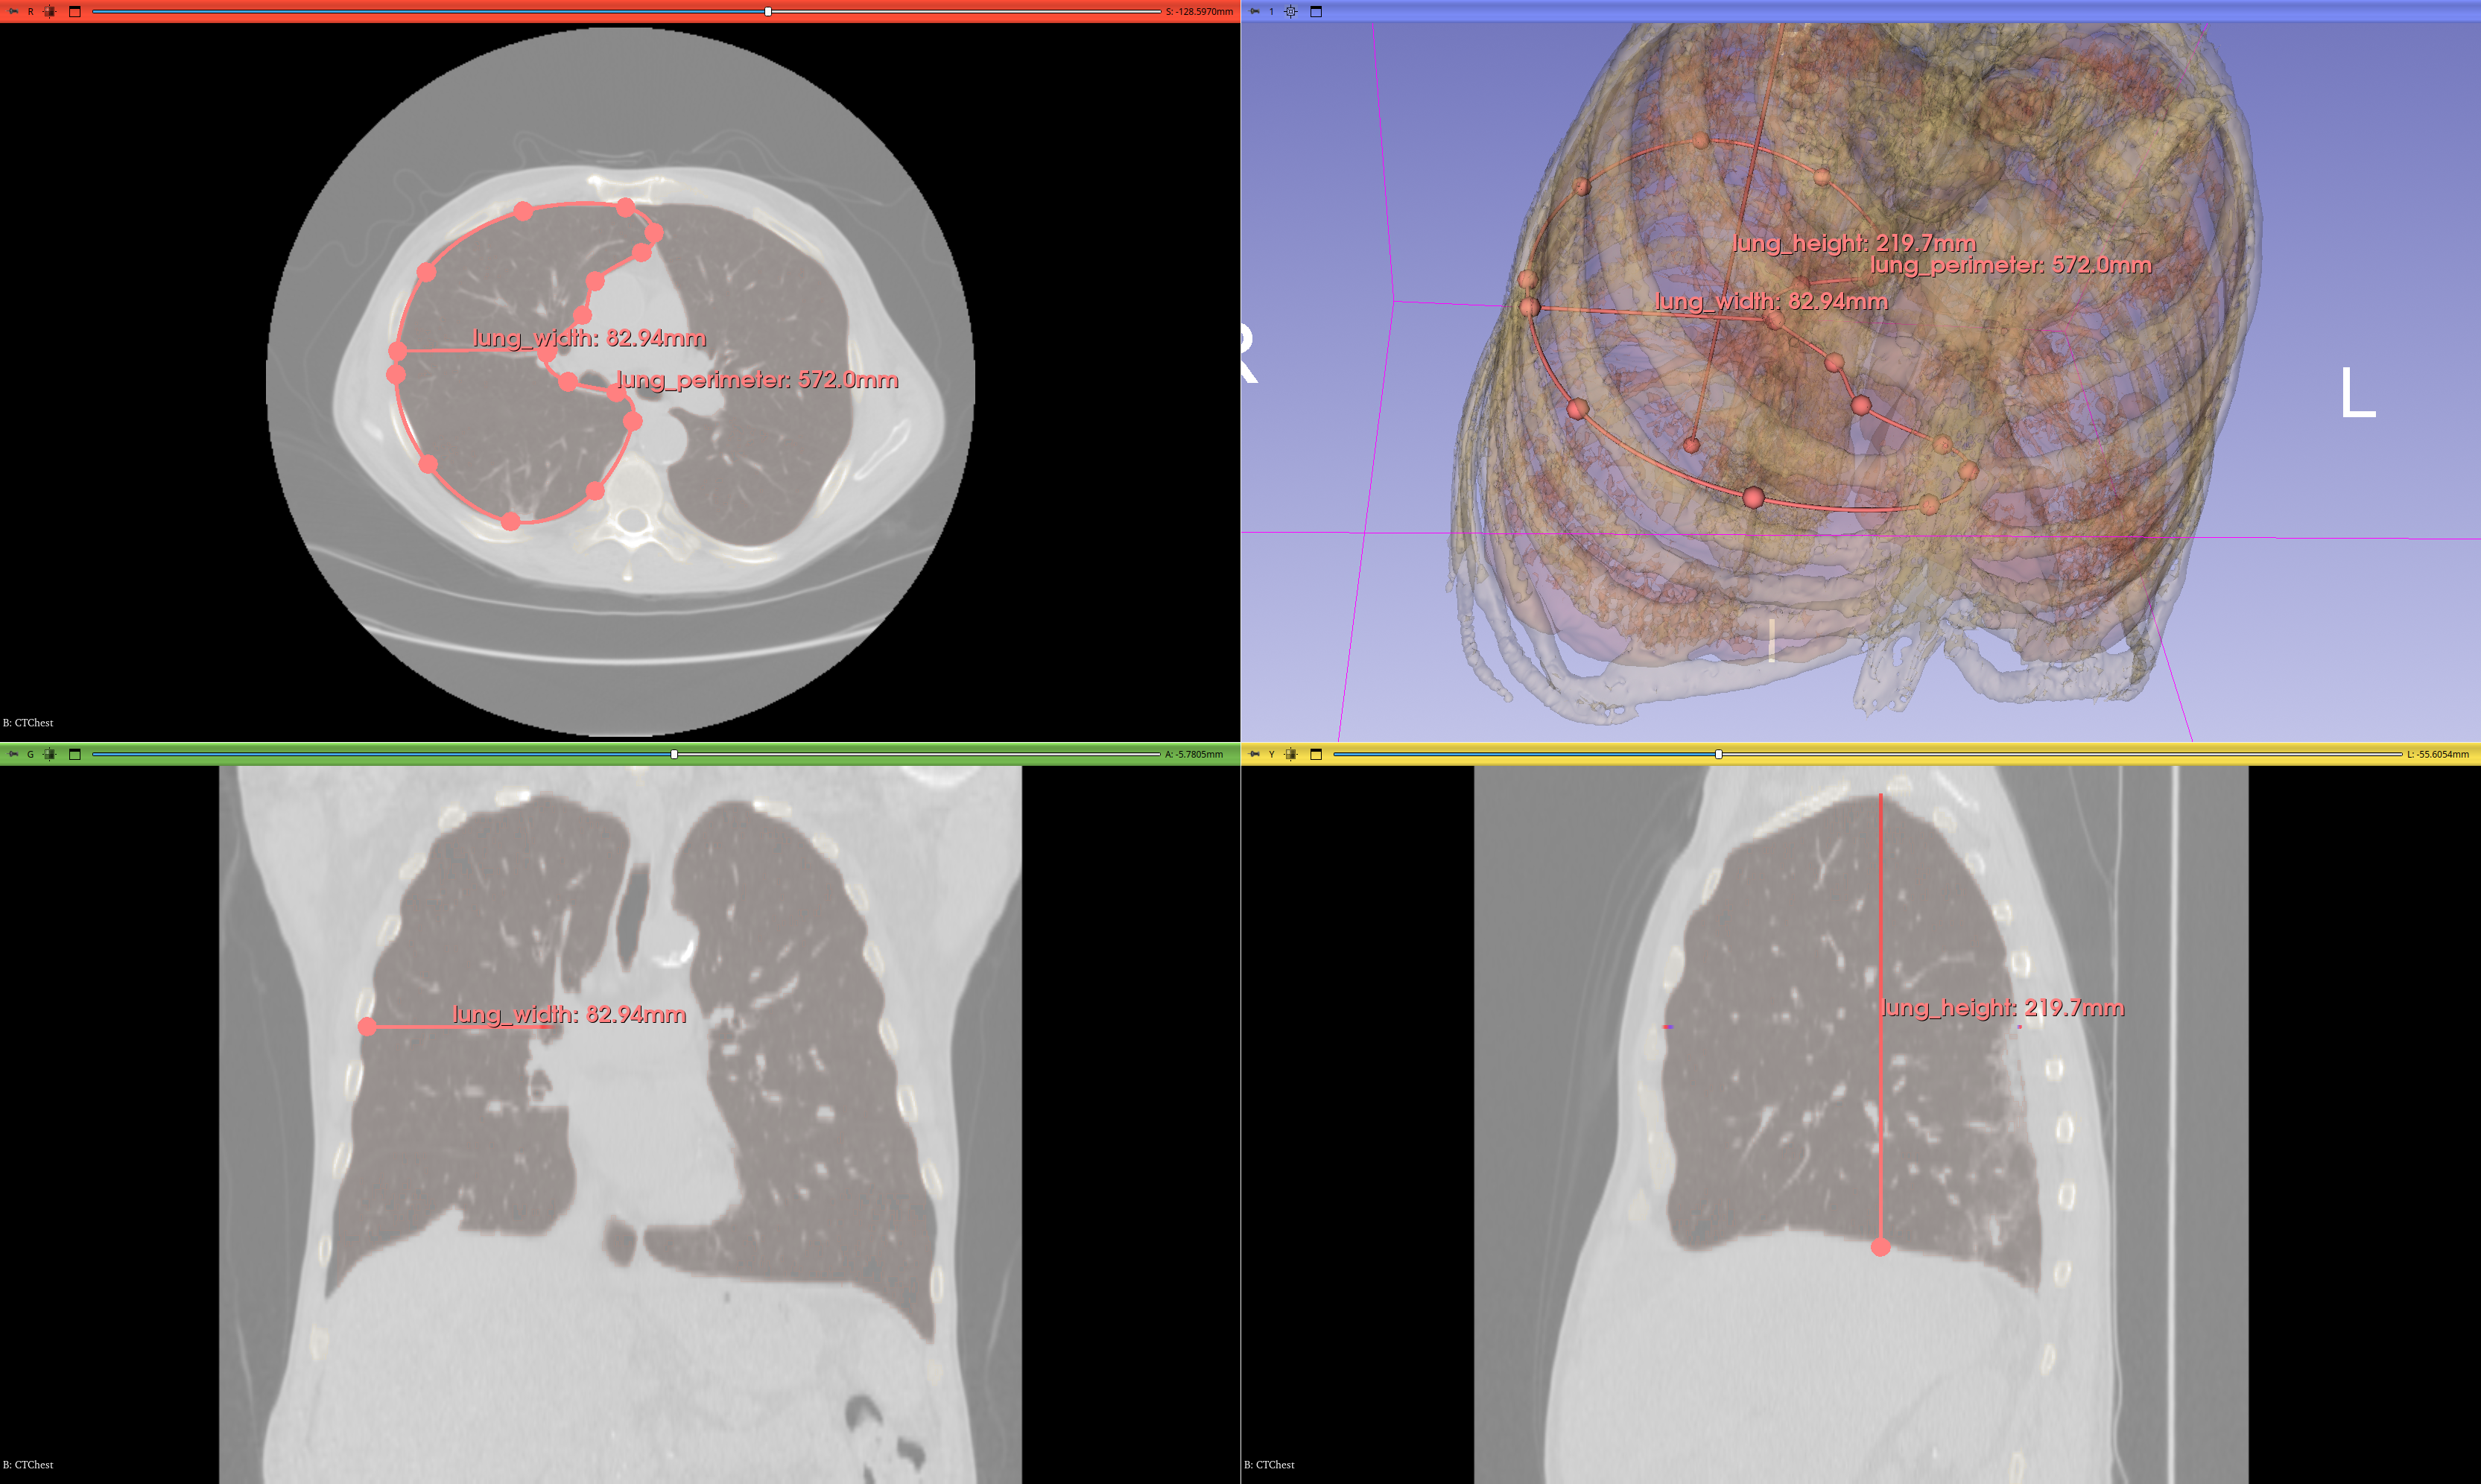
\includegraphics[width=0.9\textwidth]{img/ex41.png}
    \caption{Combined visualization of the lungs segmentation, anatomical 2D views, and measurements.}
    \label{fig:report_task}
\end{figure}

In order to enhance the visualization of the perimeter markups, the opacity of the segmentation model was reduced, leading thus, a clearer view.
